
Due to the ever-increasing volume of data, there is an urgent need to provide expressive and efficient %data analytic tools. 
tools to support Big-Data analytics.
%Datalog, a declarative logical programming language, 
%has been widely implemented  due to its superiority of concise expressing and efficient execution of recursive queries. 
The declarative logical  language BigDatalog %implementation on Apache Spark system, BigDatalog, 
has proven very effective at expressing concisely graph, machine learning, and knowledge discovery applications via recursive queries that execute with superior 
performance and scalability  on  Apache Spark. 
% via concise recursive queries for graph, machine learning, and knowledge discovery applications
% with superior scalability of Spark system.
To help data scientists benefit from these advances in full synergy with  Spark's rich libraries and programming environs, we develop the  Spark DataFrame extension LFrame and the Logical Algorithm Library  LLib.
LLib provides a wide range of Datalog algorithms written using BigDatalog  on Apache Spark. LLib encapsulates complex logic-based algorithms into 
high-level APIs, which simplify the development and   provide a unified interface akin to the one of Spark MLlib.   As a fully compatible
DataFrame-based API, LLib enables the integrated utilization of LLib 
applications and new Datalog queries with existing Spark functions, such 
as those provided by MLlib and Spark SQL. 
% ?allows these algorithms jointly utilized with all existing
%is proposed to be  DataFrame-based so that it can flexibly collaborate with existing
% Spark functions such as those provided by MLlib and Spark SQL.  
%via LFrame which is a fully compatible
%extension of Data Frames.
%Considering the requirements for developing novel recursive applications not contained in LLib, 
To facilitate the development 
of new applications not contained in LLib, our system provides an 
LFrame-based  programming interface to Datalog.
LFrame objects convert directly to and from DataFrame objects to support both relational operations and  logic-based operations. 
In addition, both LLib and LFrame support interoperability with multiple programming languages, whereby users can now  express  succinctly powerful recursive queries in 
Scala, Java, or Python. 
As a result, BigDatalog becomes a very attractive software development tool in the Apache Spak ecosystem. 
This chapter utilizes several running examples to demonstrate the  power and versatility of LLib and LFrame.

\section{Introduction}
In the era of big data, the demand for flexible analytics on large-scale data has driven researchers to build various general-purpose user-friendly platforms like Apache Spark   \citep{zaharia2012resilient}, AsterixDB \citep{alsubaiee2014asterixdb}, Pig \citep{olston2008pig}, Hive \citep{thusoo2009hive}, etc.  Among these systems, Spark is getting more and more attractive due to its efficient in-memory computation and abundant APIs (i.e. Spark SQL, GraphX, MLlib and SparkR) for sophisticated analytics  to extract rich information encapsulated in the data.

However, for iterative applications like identifying transitive closures or connected components of millions of vertexes, there are no dedicated designs for optimization among recursions in Spark.
% in Spark because each iteration is contained in an identical job.  
For  more sophisticated recursive analytics, the programming needs deep understanding and extensive knowledge of the platform.  To solve these issues, researchers have attempted to implement Datalog  \citep{consens1990low} systems. 

Datalog, a well known logical programming language with superior expressive power on recursive algorithms, consists of a set of rules and facts. The DeALS project of UCLA \citep{yang2015parallel} implements a unified Datalog programming language and provides a parallel evaluation on multi-core machines. For the distributed logical computing on clusters, the BigDatalog \citep{shkapsky2016big} system is further developed on Spark. While considering the SQL programming customs, the Recursive-aggregate-SQL (RaSQL) \citep{gu2019rasql} is proposed as a simple extension of Spark SQL for Datalog.  


% Similarly, other systems also do not support efficient iterative computing or a unified logic-based language for concise expression. 
This torrent of Datalog platforms, however, underscores the needs to make Datalog as an integral part of data processing pipeline and provide high-level APIs to simplify the development. % and the usage of logical programming as an important step within the data processing pipeline. 
In those systems, one Datalog application run independently as one  job with input rules and datasets. It requires much programming for users to convert the output of one Datalog program to the required input of another Datalog program. Similarly, the collaboration with other libraries like machine learning (MLlib), graph computation (GraphX) in Spark is inconvenient. Also, it is necessary for users to learn about Datalog or get used to a SQL extension (RaSQL) when they actually  want a simple function wrapping all the logic of a common Datalog algorithm. 


In this chapter, we focus on making the Datalog module as the first-class citizen in Spark, that can easily collaborate with Spark libraries. We proposes LLib, wrapping all key Datalog algorithms with a unified interface for adding new ones, and LFrame, the DataFrame extension supporting the logical operations.  LLib and LFrame are implemented on BigDatalog and Spark. They can support multiple programming languages, such as Python, Scala and Java. The wide audience of Spark community should be familiar with the interface of LLib (like Spark MLlib) and LFrame (like Spark DataFrame). With LFrame and LLib, data scientists could have access to the data manipulated in Datalog applications and  continuously do subsequent processing like machine learning algorithm within one job. 
This ecosystem makes the end-to-end developing Datalog algorithms with a high-level API (LLib) possible. For a user-defined recursive application outside LLib, with LFrame, it can be as friendly as Pandas~\citep{mckinney2010data}/Spark DataFrame. 
% possible to ask for help from the existing Datalog algorithms by solely a one-line function calling within a processing pipeline and 
% develop user-defined recursive application as friendly as the Pandas\citep{mckinney2010data}/Spark DataFrame. 

Our contributions can be concluded as following:
\begin{itemize}
	
	\item Usability. Both LLib and LFrame are tailored to data scientists and support multiple programming languages including Python, Scala and Java. In addition, LLib  provides functions for a wide range of typical Datalog algorithms and makes it possible for the end-to-end  recursive development  with high-level APIs.
	% and avoids the efforts required to learn a new language syntax. 
	\item Interoperability. LLib is the DataFrame-based API, which takes the DataFrames as the input and generates also DataFrames. This facilitates the collaborations between LLib applications and Spark MLlib, Spark SQL or GraphX. As for LFrame, we provide the functions for flexible conversions between the  DataFrame and LFrame, which also smooth the collaborations between LFrame-basesd algorithms and Spark libraries. Both LLib and LFrame make the Datalog module as an integral part of data processing pipeline. 
	\item Extendability and flexibility. In LLib, there is a template and several utility functions to help  contributing extra Datalog algorithms. We also allow user-defined Datalog function on LLib to wrap any possible Datalog algorithm.  LFrame data structure is associated with various general Datalog operations to develop any recursive algorithm.
\end{itemize}
The chapter is organized as follows. Section \ref{pre} reviews the basics about the Datalog language and related platforms including Apache Spark, BigDatalog and RaSQL. Section \ref{llib} describes the working paradigm of LLib,  
user-defined Datalog functions and the collaborations with other Spark libraries. 
Section \ref{lframe} presents the conversion between LFrame and DataFrame, the basic unary and $N$-ary operations supported by LFrame, and some examples by LFrame. Section \ref{multi} demonstrates our design to support multi-language programming. Section \ref{sec:libperf} discusses the performance overhead. Section \ref{conclusion} draws  conclusion and maps out plans for future work.

\section{Prelimiaries}
\label{pre}
\subsection{Datalog}
% base case, recursive case,
A Datalog application is comprised of a finite set of rules. Each rule $r$ is formed as H $\leftarrow l_1, l_2, ... l_n$, where H is the head of $r$, $l_{1..n}$ (the \textit{body}) are \textit{literals}   and the $\leftarrow$ means implication. The literals ($l_{1..n}$) are positive or negated atoms. One atom (H or $l_i$) can be formed as $p(t_1, .., t_k)$, where $p$ is a \textit{predicate} and $(t_1, .., t_k)$ terms can be \textit{variables}, \textit{constants} or \textit{functions}. So, the $r$ is a rule to infer H. However, if $r$ does not have the body $l_1, l_2, ... l_n$, it becomes the \textit{fact}, which corresponds to a tuple in a relation . The comma separating literals means the logical conjunction (AND). To evaluate a Datalog application, we need a \textit{query} indicating which predicate to evaluate.

Next, we will illustrate a classic example in Datalog, single source shortest path (SSSP),  with more terms covered below. The SSSP is to calculate the length of shortest paths from one source vertex to all other vertices in a graph with weighted edges. 

\vspace{0.5em}
\qr{1} - Single source shortest path (SSSP).
\setcounter{myrow}{0}
\\
$\begin{array}{>{\quad \stepcounter   {myrow} \themyrow : \quad}lrl}

database(\{\ warc(A: integer,\  B: integer,\ Cost: integer)\ \}). \\

sp(B,\ mmin<C>) \leftarrow B=\{startvertex\},\ C=0. \\

sp(B2,\ mmin<C>)\leftarrow sp(B1, C1),\ warc(B1, B2, C2),\ C=C1+C2. \\
result(B,\ min<C>) \leftarrow sp(B, C). \\

query\ result(T, C).


\end{array}$
\vspace{0.5em}

As shown in Query 1 line 1, the input relation (\textit{base relation}) is \textsf{warc} with the schema \textsf{(A:integer, B:integer, Cost:integer)}. 
One fact of this relation can be \textsf{warc(1, 2, 5)}, which shows the  cost from   the vertex 1 to 2 is 5. The \textsf{database} is a keyword specifying the base relation.
In the first rule (line~2), it initializes the shortest distance from the source vertex to itself as 0, where the ``\{startvetex\}'' can allow user to input the source vertex ID. The second rule (line~3) recursively produces all the minimum distances for all possible paths from source node to another node. The monotonic aggregate \citep{zaniolo2019monotonic,das2019bigdata}, \textsf{mmin} is utilized, which allows the aggregation inside the recursion when set containment is satisfied. The \textsf{mmin} will get a new lower value with a larger set of possible paths. And a normal aggregate \textsf{min} is finally exploited (line~4) to obtain the minimum cost path. The fifth line denotes the  predicate (\textit{relation}), \textsf{result(T,C)} will be evaluated and become the output of the application.

\subsection{Related Platforms: Apache Spark, BigDatalog and RaSQL}
\textbf{Apache Spark.} Apache Spark is a DISC system with various modules like Spark SQL \citep{sparksql},  MLlib \citep{meng2016mllib} and GraphX \citep{gonzalez2014graphx} to support analytics on structured data, machine learing algorithms and graph computation algorithms respectively.  All the Spark applications are eventually represented by a series of transformations and actions on Resilient Distributed Datasets (RDDs) \citep{dean2004mapreduce}, the main abstraction provided by Spark. The operators like groupBy and filter are lazily evaluated until an output action like count trigger evaluations on RDDs. In this way, before execution, the Spark Optimizer can design a better physical plan by avoiding some duplicate computation or pipelining operations. RDDs in Spark are actually Python or Java objects stored in memory and can be processed in parallel. %Unlike RDD, the Spark DataFrame organize  data  into named columns.
% The RDD is fault-tolerant due to its lineage. The lineage graph of RDDs records the transformations applied to them.  The Spark has attracted wide audiences from database community due to its high usability and performance.

\textbf{BigDatalog.}
With the popularity of Spark and the benefits for recursive query evaluation and optimization brought by Datalog, the new requirements have been re-emerged to support the Datalog programming on Spark. 
As far as we can find, BigDatalog \citep{shkapsky2016big} is the first platform implementing DeALS, a Datalog platform, on Spark. It supports the execution of recursive operations on  multi-core machines and clusters. BigDatalog also proposes optimizations on physical planning for recursive queries to obtain performance improvement. 

\textbf{RaSQL.} 
BigDatalog enables development of Datalog on Spark, but users should get used to the Datalog syntax. With the continuing popularity of SQL, it is beneficial to design a language similar to SQL for Datalog queries. RaSQL \citep{gu2019rasql} proposes a new language following and extending SQL standards, and utilizes some novel optimizations on fixpoint operators for the Datalog platform built on Apache Spark.  

% Development of a Datalog application on BigDatalog or RaSQL  consists of a query file, a structured data file, and a standard execution program, which takes the query and data files with some arguments for execution. Users need to learn Datalog or RaSQL syntax and it is not so interoperable  between one Datalog application and another Spark MLlib, Spark SQL or Datalog application. In this chapter, we would like to  introduce the LLib and LFrame to  simplify the development.


\subsection{Spark MLlib and DataFrame}
% AFrame, DataFrame in Panda and Spark, R

MLlib is the machine learning library of Spark. It consists of classification and regression algorithms. Users can flexibly build a pipeline of a sequence of algorithms to process data with the abundant libraries in MLlib. The pipeline could span across data cleaning, model initialization, training, prediction, and evaluation.  

DataFrame is a popular facility for data scientists and has been supported by various trendy data analytics platforms and languages such as Spark, Pandas~\citep{pythonDataframe}, R, etc. It is utilized as a data structure and the data stored there is organized in rows and columns like a table in Excel. This increases the visibility of development for non-expert users. The supported operations for the DataFrame are similar to the relational algebra, but are exposed as pre-defined functions like libraries of Java, Python, etc.  


 
\section{LLib}
\label{llib}
In this section, we discuss LLib, which works in a similar way as MLlib to develop Datalog applications. It does not require  users to be familiar with logical programming. LLib contains a wide spectrum of recursive applications including graph algorithms (Transitive Closure, i.e. \textit{TC}), temporal database queries (Interval Coalesce), financial applications (MLM),  machine learning algorithms (Logistic Regression), etc. 
The data analysts could easily take one Datalog algorithm as one step within their complex data processing process, which is more flexible than the previous Datalog programming interfaces. 











\subsection{Working Paradigms Comparison: LLib, BigDatalog and RaSQL}
\label{sec:paradigm}
% Schema Mapping, Single DataFrame, Multiple DataFrame, Different outputs format, Arguments (Start Vetex =?)
% Wrapped DatalogSession, No need for arguments (configuration)

LLib grants the access to the processed data to users through the Spark DataFrame, which greatly reduces the required boilerplate code and improves  the readability. In this part, we would like to firstly provide a high level picture of the differences while working on two popular Spark-based distributed Datalog platforms (BigDatalog and RaSQL) and our LLib. 

As shown in Figure \ref{fig:comparison} (a) about Transitive Closure application, the previous Datalog programs are made up of (1)  source data file(s), which should follow a determined format, (2) a query file following RaSQL or BigDatalog syntax, (3) a standardized program (script) to execute the query on the source data, and (4) a set of arguments to guide the execution. This is a general-purpose design for all potential applications that can be expressed by a combination of rules running on several data files, but it causes a troublesome programming considering the following aspects.


\begin{itemize}
	\item \textit{Learning new language.} Users are required to learn the syntax of Datalog or an extension of SQL while they actually  want to use a well-wrapped Datalog function.
	\item \textit{Data preparation.} For each application on the previous platforms, the required data need to follow a determined format. It costs extra time for the data preparation.
	\item \textit {Isolation from other applications.} The development mode  of the original logical programming works in a way like a black box. Users provide data and rules to standardize program and get results. They only have access to the generated file and can hardly involve  preprocessing or subsequent processing.  
\end{itemize}

To tackle those issues, we develop the DataFrame-core LLib as shown in Figure \ref{fig:comparison} (b), where Datalog applications are seamlessly integrated into the data processing pipeline. Within an LLib-based application, there can be many steps made up of the permutations of regular DataFrame operations,  MLlib's ML algorithms and LLib's Datalog algorithms. Users do not need to manually program to connect $s_1$...$ s_n$ by preparing Datalog input data or persisting and loading Datalog execution results for subsequent processing.  Later in next subsection, we will describe the underlying architecture and working pipeline of LLib through a running example, Transitive Closure. 

\begin{figure}[!t]
	\centering
	\begin{subfigure}{0.7\textwidth}
		\centering
		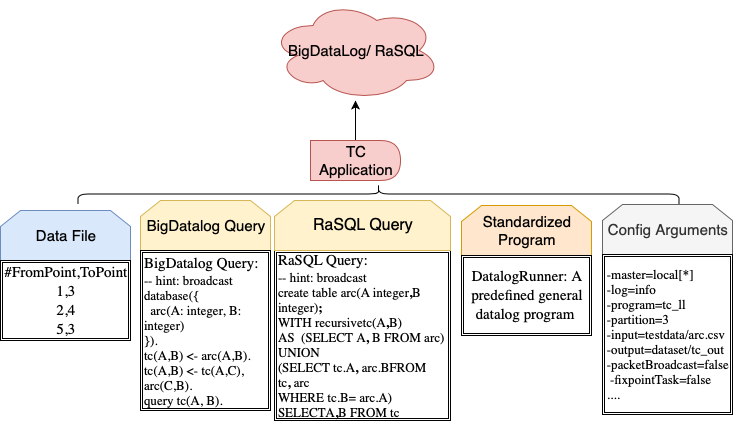
\includegraphics[width=1\linewidth]{Graph/llib/datalogPipeline.png}
		\caption{\small The composition of TC application on custom Datalog platforms. } 
	\end{subfigure}%
	%   \hspace{1em}
	\vspace{\floatsep}
	
	\begin{subfigure}{0.6\textwidth}
		\centering
		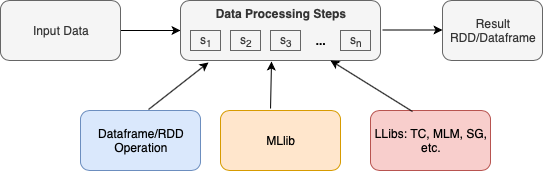
\includegraphics[width=1\linewidth]{Graph/llib/DatalogLib-4.png}
		\caption{\small LLib paradigm} 
	\end{subfigure}%
	\caption{Working paradigm comparison between existing Spark-Based Datalog platforms and LLib.}\label{fig:comparison}
	\vspace{-1em}
\end{figure}


\subsection{LLib Processing Pipeline and Underlying Architecture}

\subsubsection{Working Session and Acquiring Data}
\label{sec:data}
In LLib, the first step is to construct a working environment for the Datalog queries and libraries. We respect the customs of building Spark Session and exploit the similar way as following (with Transitive Closure, i.e. TC as a running example):


\vspace{0.5em}
\ex{1.1} - Transitive closure with LLib:  Working session.
\bldl
session = LLibSession.builder(
).appName(``TC").master(``local[*]"
).getOrCreate()\\

schema = StructType(List(StructField(``Point1", IntegerType, true),\\
StructField(``Point2", IntegerType, true)))\\

df = session.read.format(``csv").option(``header",``false").schema(schema)
.load(``arc.csv")
\eldl
\textit{LLibSession} synthesizes the  Spark environment and the special designs for logical programming. Within the same session, users are free to utilize existing Spark libraries like data loading functions to create a DataFrame \textit{df} (line 4)  or our Datalog libraries i.e. LLib or LFrame. 
% As shown in the forth line, the source data can be loaded via the loading function in Spark to a DataFrame \textit{df}. 

\subsubsection{Initializing an Executable Object of LLib and  Mapping the Schema}

\textbf{Initialization: }In LLib, the pipeline of the data processing for a typical application is wrapped to an executable object, which users can initialize and set parameters of. In Example 1.2, we initialize a transitive closure object tc with the TC library, which is pre-defined and included in the LLib. 
Then, we can set the property by built-in functions. 


\vspace{0.5em}
\ex{1.2} - Transitive closure with LLib:  Initializing TC.
\cldl
import\ edu.ucla.cs.wis.bigdatalog.spark.LLib.TC \\
val\ tc = new\ TC() \\

tc.setDirection(FromCol = "Node1", ToCol = "Node2")
\eldl

\vspace{0.5em}
\qr{2} - Transitive closure.
\bldl
database({
	arc(From: integer, To: integer)
}).\\


tc(From,To) \leftarrow arc(From,To).\\
tc(From,To) \leftarrow tc(From,Tmp), arc(Tmp,To). \\
query\ tc(From, To).
\eldl

\textbf{Schema Mapping: }Among the built-in functions,  all the libraries are required to contain one function \textit{setDirection} for schema mapping. This is necessary because we want a more general design to accept   DataFrames with various schemas as the input.  
One attribute may have different names in different DataFrames. With schema mapping, we could know the corresponding relationship between input DataFrame's attributes and the attributes in our library's computing logic.
% DataFrame may call an attribute with an arbitrary name but we need to know the corresponding relationship between its attributes and the attributes in our library's computing logic. 
For example, Query 2 is a set of Datalog rules used by the transitive closure of our library. We have two attributes,  From and To, in the arc table. The two attributes can be called differently like (Node1, Node2) as shown in the df initialized in Example 1.1. The mapping between (From, To) and (Node1, Node2) can be provided by the setDirection function as shown in the third line of Example 1.2. If there is a long mapping list for attributes, we can store the mapping information within a hash table.


\textbf{Schema Recovering:} While processing the data with our library, we need the mapping information. But after processing, the output data's format should be consistent. There is one mechanism to rollback the schema. At the beginning of data processing, we store the schema of the input data. Then, in the end, we could use the pre-stored schema to recover. 

% When the amount of required attributes by the library matches the amount of columns in the input DataFrame, we could  make full use of the dataset. However, when the dataset contains more attributes than the required, it should be pruned before analysis. As for the condition that the required attributes not included or the dataset contains fewer attributes than  the required, exceptions will be raised.



\subsubsection{Execution and Persistence}
With the executable object and imported data, the execution and persistence can be merely a one-line execution with a pre-defined function (run, genDF or genRDD) in LLib. These three functions can support basic requirements to operate data and store the result to a variable or a file. As shown in Example 1.3, the function $run$ is to run the logical programming and persist the result directly to the target address. If users would like to do subsequent processing, it can output the data into a DataFrame or RDD as shown in  second and third line of the Example 1.3. 

\vspace{0.5em}
\ex{1.3} - Transitive closure with LLib:  Execution and persistence.
\bldl
tc.run(df, output = "File", session) \\
val\ dfNew = tc.genDF(df, session) \\
val\ rddNew = tc.genRDD(df, session) \\

\eldl


These three functions are implemented for each library of LLib. They expect the input data (df) and the environment (session) as inputs.  The session information is needed for during execution, we want the program running in an environment with ability to support logical
programming. 


\subsubsection{Multiple Data Sources}
\label{sec:multiple}
The previous TC example operates on only one relation, however there are many applications requiring more than one relation, which brings changes to the  pipeline. We illustrate the Multi level Market (MLM) Bonus as a typical Datalog application \citep{mlm} acquiring more than one dataset. The application is to calculate the bonus for members of a hierarchical structural Multi Level Marketing  organization. In the organization,  new members are recruited by  and get products from old members (sponsors). One member's bonus is based on his own sales and a proportion of the sales from the people directly or indirectly recruited by him. The  scale of the proportion is user-defined. 

There are two relations in MLM Bonus, including the \textit{sponsor} and \textit{sales}. The sponsor relation describes the recruiting relationship among members, while the sales relation records the profits for each member. In  Datalog syntax, the base case should be calculating the member's bonus by the sales table. And the recursive rule is to calculate the bonus based on the basic profits and the profits derived from the downstream members.

With the help of LLib, users could implement MLM Bonus by a pre-defined class in LLib  ignoring the complex logic. The program can be as easy as  follows.

\vspace{0.5em}
\ex{2} - LLib with more than one input relation: Multi level Market Bonus.
\bldl
val\ MLM = new\ MLM() \\
MLM.setDirection(MCol = "Member", ProfitCol = "Bonus")\\
MLM.setSecDirection(MCol = "Member1", M2Col = "Member2") \\
MLM.run(Array(dfSales, dfSponsor), output = "resMLM", session) \\

\eldl
Suppose we already have the two relations stored in dfSales and dfSponsor. In the first line, we build an executable object of MLM. Then, we set the schema mappings for two relations in the next two lines. To operate the data and persist to resMLM file, we use the forth line with the run function.  The run function of previous TC application only expects one relation as the input. While dealing with multiple relations, we aggregate the relations in an array as the input. The schema mapping is implemented by adding a new function for the second relation. However, it is possible to  maintain the schema mapping for each relation in a hash function ($h_r$) and use another hash function with the relation's name as the key and the schema mapping information (the hash function, $h_r$) as the value. 
% to store the mapping between the relation and the schema mapping hashing. 
\iffalse
\subsection{LLib Categories}
The supported common Datalog algorithms and utilities in LLib can be  categorized into five groups. We briefly introduce each group and the typical algorithms. 

\textbf{Graph algorithms:} The most common cases of recursive computations  belong to the graph algorithms. In LLib, the typical graph algorithms are Single Source Shortest Path (SSSP), Transitive Closure (TC), Connected Components (CC), and Count Paths (CP). The SSSP  computes the shortest paths from a specific source vertex to all other nodes in a graph with weighted edges. The length of paths are computed iteratively and there is a min aggregation to choose the shortest one. The usage of the SSSP from LLib is as follows.

\vspace{0.5em}
\ex{3} - A graph algorithm (SSSP) supported by LLib.
\bldl
val\ SSSP = new\ SSSP() \\
SSSP.setFromVertex(vertexID = 1) \\
SSSP.setDirection(fromCol = "From", toCol = "To", costCol = "Cost") \\
SSSP.run(df, output = "resSSSP", session) \\

\eldl
The program differs from the TC example on the second line, where the source vertex is set. The remaining part of the program is identical to TC, which has been fully explained previously. 

CC is to identify the connected components of a graph by attaching and updating each node with a group ID in iterations. The group ID is set each time as the minimum node ID among the nearby nodes. The nodes in a connected component will finally share the same group ID and we just need to compute the number of distinct group IDs. In CP algorithm, we obtain the number of paths from one node to  the other nodes in a graph. The reachability  is transferred iteratively along the edges of graph. The development with CC and CP library will be similar to the TC library, where only the schema mapping is required before execution. 

\textbf{Machine learning algorithms:}
Another series of algorithms, which can be expressed by Datalog queries, are  machine learning algorithms.  Previously, the development for a simple algorithm like Linear Regression or Logistic Regression needs the intensive understanding of the Datalog. With inspirations from Spark MLlib, we provide a more declarative way to develop the machine learning algorithms (including logistic regression, linear regression, SVM, etc.)  on the Datalog platform. 
% We have shown the ML algorithms can be expressed with Datalog, but to attract a wider audience of the data science, it is important to provide a more elegant and succinct way like Spark MLlib. We provide a high-level API for the common ML algorithms including linear regression, logistic regression, etc. 
To illustrate the development with our API, we show a running example exploiting the logistic regression class.

\vspace{0.5em}
\ex{4} - Developing machine learning algorithms with LLib.
\vspace{-2em}
\bldl
//\ Import\ data. 
\\
var\ Vschema = StructType(List(StructField("Id", IntegerType, true), \\StructField(
"C", IntegerType, true),
StructField("V", DoubleType, true),\\ StructField("Y", IntegerType, true))) \\

var\ df = spark.read.format("csv").option("header", "false").schema(Vschema).load("dataV") \\
\\
//\ Training\ on\ the\ input\ relation\ df. \\
import\ edu.ucla.cs.wis.bigdatalog.spark.LLib.DL\_LogisticRegression \\
val\ lr = new\  DL\_LogisticRegression().setMaxIter(10) \\
val\ lrModel = lr.run(df, session)

\eldl
The running environment of our program is still the LLibSession. Then, we can load a pre-processed training dataset stored in a verticalized view with \textit{Vschema} (Id, F, V, T), where the Id is the identification of each training instance; the F is the feature's ID; the V is the feature's value and the T is the label. The verticalized format is beneficial for sparse training data and the transactions of Datalog rules.   After importing the required training functions for logistic regression, we could build an executable training object, \textit{lr}. The \textit{lr} wraps all the logical rules and some required relations (e.g. parameters with default value 0) of the Datalog implementation for the logistic regression training.  While initializing the lr, users can exploit the built-in functions to set the properties like the limit of  iterations, the intial value of parameters, etc. During training (\textit{run}), the session information of the Datalog environment is also required. 
% After fitting the model to \textit{df} relation, the \textit{transform} could make predictions on the testing instances with the pre-trained model \textit{lrModel}.

For comparison, we leverage the Spark MLlib for the above example. The development will become the following, which looks very similar. The differences are: 1)The  input data (\textit{dataS}) do not need verticalization and the schema is not the \textit{Vschema}; 2) An assembler is leveraged to specify the attributes belonging to the features, while in LLib, the verticalized relation is self-explanatory.; 3) The session information is not required during training, while in LLib, the session should be one input parameter for training.
Even though the differences exist, the expressing with Spark MLlib and LLib are extraordinarily similar and both user-friendly.

\vspace{0.5em}
\ex{5} - Machine learning algorithms training with Spark MLlib.
\bldl
//\ Import\ data. \\
var\ schema = StructType(List(StructField("X1", IntegerType, true), \\StructField(
"X2", IntegerType, true),
StructField("X3", DoubleType, true),\\ StructField("label", IntegerType, true))) \\

var\ df = spark.read.format("csv").option("header", "false").schema(schema).load("dataS") \\
\\
//\ Training\ on\ the\ input\ relation\ df. \\
import\ org.apache.spark.ml.Pipeline \\
import\ org.apache.spark.ml.classification.LogisticRegression \\
import\ org.apache.spark.ml.feature.VectorAssembler
\\
val\ assembler = new\ VectorAssembler()
.setInputCols(Array("X1", "X2", "X3"))\\
.setOutputCol("features") \\
val\ lr = new\  LogisticRegression().setMaxIter(10) \\
val\ pipeline = new\ Pipeline().setStages(Array(assembler, lr)) \\
val\ lrModel = pipeline.fit(df) \\
\\
% \\
% //\ Testing\  with\ pre-trained\ model. \\
%     var\ test = spark.read.format("csv").option("header", "false").schema(schema).load("test") \\
% val\ prediction = lrModel.transform(lrModel, test)

\eldl


% Before loading the data, the relation should have been stored in a verticalized view with schema (Id, C, V, Y) as introduced in Section 3.1. 

\textbf{Temporal database queries:}
LLib also supports the transactions on data related to time. For example, in the Interval Coalesce, the goal is to find the smallest set of intervals to cover the input intervals. In Datalog, users are supposed to exploit one rule to find the start points (\textit{S}) of intervals which are not inside the other intervals and another rule to recursively extend the right side of intervals, whose left side belonging to \textit{S}. However, in the LLib, the development will be as simple as follows with \textit{df} (S and E column represents the start point and end point) as the input intervals and the \textit{session} built by LLibSession.


\vspace{0.5em}
\ex{6} - Temporal database query with LLib.
\bldl
val\ Coalesce = new\ Coalesce() \\
Coalesce.setDirection(startCol = "S", endCol = "E") \\
Coalesce.run(df, output = "res", session)
\eldl

\textbf{Financial   applications:}
Except the MLM Bonus mentioned in Section \ref{sec:multiple}, we also support the other financial applications like Bill of Matreials (BOM) \citep{BOM} and  Management. In BOM, one input relation is \textit{assembling} table recording the assembling relation between one item $i$ (or a part of $i$) and its immediate subparts. Another input is \textit{basic} table recording the time cost to deliver the basic parts. The task can be calculating the days required to get  the $i$ ready. We can obtain the required time for each subpart of $i$ and use the maximum time as the result. The calculating of time for each subpart of $i$ should be  execute recursively. In Management, the input table stores the manager and the employees managed by them, and the task is to calculate the total account of employees directly or indirectly managed by one manager. This also requires recursive execution. In LLib, we provide a class wrapping the execution of the BOM or Management and the usage will be similar to the example introduced in Section \ref{sec:paradigm}.

\textbf{Other applications:}
Some other important and classical recursive query applications are also contained in LLib, like same-generation (SG), which identifies pairs of humans with the same hop distance to a common ancestor.  The working paradigm with them will be similar to the Spark MLlib and same as the examples in Section \ref{sec:paradigm}. Here, we will not make repetitive illustrations.
\fi
\subsection{Extension of LLib}
Besides a wide range of custom recursive algorithms, LLib also provides a unified template, \textit{TempLib}, to follow when followers contribute  new algorithms. 
% All existing algorithms are developed based on the TempLib. 
TempLib contains abundant utility functions to facilitate development and some requirements to follow. %The implementation should at least include three functions (run, genDF and genRDD) for execution and persistence. 
With the template, the implementation becomes quite uncomplicated. As long as users have the Datalog rules for the algorithm, they can add their own algorithm by doing minor changes to the existing codes for algorithms like TC. 


\subsection{Collaboration with Other Applications}
The input and output relations in LLib can be both DataFrames, which makes it possible to add a preprocessing algorithm which generates the input DataFrames  or  a subsequent processing algorithm which takes the DataFrame generated from LLib. LLib allows users to exploit the Datalog application as a simple step at any place of their  processing pipelines. In this section, we illustrate with a concrete example to show the collaborations between LLib and other applications like Spark MLlib or Spark DataFrame Operations. The showed LLib application is the MLM Bonus application mentioned previously, and we want to use the linear regression library from MLlib to get the relation between the bonus and the working days for a member. To save space, we do not show the process to build the session (LLibSession), and load input relations (dfSales, dfSponsor, dfWorkTime).  The dfWorkTime stores the working days for each member. With MLM class from LLib, we could get the \textit{dfRes} storing the bonus for each member. Joining the result relation with the dfWorkTime on the member column will generate a new relation with columns of the day and bonus. The Linear Regression function from MLlib could train on the result DataFrame. In this example, we can find the  LLib is able to collaborate fluently with other operations in Spark like MLlib (LinearRegression), DataFrame Operations (join). Similarly, the collaboration among multiple Datalog applications is also possible.  

\vspace{0.5em}
\ex{3} - Collaboration between LLib and other Spark libraries.
\bldl
val\ MLM = new\ MLM()\\
MLM.setDirection(MCol = "Member", ProfitCol = "Bonus")\\
MLM.setSecDirection(MCol = "Member1", M2Col = "Member2") \\
val\ dfRes = Delivery.genDF(Array(dfSales, dfSponsor), session)\\
val\ dfRes = dfRes.join(dfWorkTime)\\ 
val\ parsedData = dfRes.rdd.map(row=>\\ LabeledPoint(
row.getAs[Int]("Days"),
Vectors.dense((row.getAs[Int]("Bonus")))
))\\
val\ numIterations = 10 \\
val\ stepSize = 0.00000001 \\

val\ model = LinearRegressionWithSGD.train(
parsedData,
numIterations,
stepSize)\\

model.save(session.sparkContext, "scalaLinearRegressionWithSGDModel")\\


\eldl



% \subsection{Multiple Datalog applications}
% A Datalog application can not only work with other Spark libraries but also work with other Datalog applications. The working paradigms of multiple Datalog applications can be in sequential or orthogonal ordering. When they work in sequence, one Datalog application will take another one's result dataset as the input. If they work in an orthogonal ordering, one application's input will be irrelevant with the data processed in other Datalog applications. Both the working paradigms can work with the LLib library, as the library operate on the DataFrame and it is simple to transfer data among applications. This cannot be achieved with the previous Datalog platforms, for they take each Datlog application as a single job to execute, which can hardly collaborate. 

\subsection{User Defined Datalog Function}
While developing, users may want to define one function (user-defined function) for once and call it many times for modular programming. To serve the user-defined datalog function (UDDF), we provide two general classes, SingleTableUDDF and MultipleTablesUDDF, which wrap the necessary components to execute the Datalog queries on single relation or multiple relations.  %The SingleTable is exploited when the UDDF has one input relation while the MultipleTables is exploited when the UUDF has more than one input relations. 
While utilizing the two classes to specify new Datalog functions, the only required information are Datalog rules and the schema of the basic table (or input table). 

\section{LFrame}
\label{lframe}
DataFrame, a widely used data structure, is always supported in different data analytic facilities like Spark SQL, Python, but not in Datalog platforms. In this section, we propose a DataFrame-like object, LFrame, wrapping the Datalog transactions and the common DataFrame transactions.
% The rest is organized as follows: Section \ref{sec:utility} describes how to convert a normal DataFrame variable to the LFrame variable. Section  \ref{sec:unary} discusses unary operations that operate on one LFrame, while the Section \ref{sec:nary} discusses the N-ary operations using with more than one  LFrame. In each of the Section \ref{sec:unary} and Section  \ref{sec:nary}, we describe one concrete example to illustrate the development with LFrame.

% In Section \ref{sec:expLFrame}, we describe two concrete examples to illustrate the development with LFrame.


\subsection{Conversion from DataFrame to LFrame}
\label{sec:utility}
% Single Frame, Different Frames
To endow a DataFrame with the ability of logical operations, we build a bridge for converting a DataFrame to LFrame. 
As shown in Example 4.1 below, the entry point of the application using LFrame is the LLibSession, same as the one in LLib, which makes it possible to use both LLib and LFrame within one execution environment. 
The session can  load the data to a DataFrame variable df, but the df cannot execute any logical transaction. To construct an LFrame variable with the  df, a built-in function wrapperDF in LLibSession can be utilized with the session and df as input arguments. 
% The session is required to obtain the Datalog running environment and the df is to supply the dataset with schema.  
% The constructed LFrame variable, lframe, could support various Datalog operations like specifying the rules, input tables, persisting the result to a file, etc. These operations are categorised to unary operations and $N$-ary operations and introduced later.

\vspace{0.5em}
\ex{4.1} - Development with LFrame:  Conversion from DataFrame to LFrame.
\bldl
val\ session = LLibSession.builder().appName("LFrame").master("local[*]").getOrCreate() \\
var\ schema = StructType(List(StructField("Parent", IntegerType, true),\\ \ StructField("Child", IntegerType, true)))\\
var\ df = session.read.format("csv").option("header", "false").schema(schema).load("sg")\\
var\ lframe = LLibSession.wrapperDF(df, session)
\eldl

\subsection{LFrame: Unary Operation}
\label{sec:unary}
The constructed LFrame in the Example 4.1 could support various Datalog operations that can be categorized to unary operations and $N$-ary operations.
The unary operation only involves one LFrame object each time. With the lframe, we implement the SG application as following to show the typical unary operations. 


\vspace{0.5em}
\ex{4.2} - Development with LFrame:  Unary operations with SG application.
\setcounter{myrow}{0}
\\

$\begin{array}{>{\stepcounter   {myrow} \themyrow : \quad}lrl}
lframe = lframe.registerCurLFrame("lframe1(Parent: integer, Chile: integer)")\\
lframe = lframe.rules("sg(X,Y) \leftarrow lframe1(Parent,X), lframe1(Parent,Y), X ~= Y")\\
lframe = lframe.rules("sg(X,Y) \leftarrow rel(A,X), sg(A,B), rel(B,Y)")\\
lframe = lframe.rules("sg(X,Y) \leftarrow sg(X,Y)")\\
lframe = lframe.delRule(3)\\
lframe = lframe.query("sg(X,Y)")\\
//\ Execution\ and\ persistence. \\
lframe.run(output = "SG")\\
val\ dfRes = lframe.genDF()\\
val\ rddRes = lframe.genRDD()
\\
//\ Normal\ DataFrame\ operations. \\
lframe.nonRecursive().where("X < 10").select("X").collect().foreach(println) \\
\end{array}$


There are five categories of unary operations included in the above example. 
\begin{itemize}
	\item \textbf{Registering one LFrame as a base relation.} In line 1, the registerCurLFrame is to register the lframe as a base relation so that the Datalog rules can utilize it as a given dataset. While registering, users are free to rename the dataset's columns and  LFrame will map the columns according to the order of appearance. 
	\item \textbf{Appending (or removing) rules.} The main body (line~2 to~4) of a Datalog program is a finite set of rules. To state the rules, the function called "rules" can be exploited. Whenever the function is utilized,  a new rule will be appended to the existing rule sets owned by the lframe.
	If one rule is wrongly appended, it can be removed by the delRule (line 5) function using its index. The provided index variable can be an array  to remove more than one rule.
	\item \textbf{Specifying the output relation.} To evaluate the application, the query function (line 6)  assists to point out the output relation, which is the sg relation in the SG. The generated result LFrame will store the output dataset in the schema specified in query, (X, Y).  
	\item \textbf{Lazy execution and persistence.} In DataFrame, the evaluation is lazy. Similarly, the LFrame's evaluation is lazy until the run action is triggered.  As shown in the second part of the code (line~8 to~10), the run function will store the result relation to a file and if a user wants to restore to a DataFrame or RDD,  genDF or genRDD function can be considered. 
	\item \textbf{Non-recursive transactions.} The design of LFrame is to wrap both the Datalog transactions and the normal DataFrame transactions. When a normal DataFrame transaction is required, like the line 12 shows, the nonRecusive function will convert LFrame to the normal DataFrame for all the DataFrame operators afterwards. 
\end{itemize}
Compare the LFrame and DataFrame, we can find they work in  analogous ways  but LFrame can support more operations. A more compact way to express the transactions from line 2 to 7 is to list them back to the lframe one by one like in line 15. 
\subsection{LFrame: N-ary Operation}
\label{sec:nary}
In the previous SG example, only one relation is contained in the Datalog application, while in this section, we illustrate the transaction (registerMoreDFs)  embroiling more relations like the join operator of the relational database. We adopt the MLM Bonus application as a running example (introduced in Example 2), for it contains both the sales and the sponsor relations. 

\vspace{0.5em}
\ex{4.3} - Development with LFrame:  $N$-ary operations with MLM Bonus application.
\setcounter{myrow}{0}
\\

$\begin{array}{>{\stepcounter   {myrow} \themyrow : \quad}lrl}
% var\ schemaAssbl = StructType(List(StructField("Part", IntegerType, true),\\ \quad StructField("Sub", IntegerType, true)))\\
%     var\ dfAssbl = session.read.format("csv").option("header", "false").\\ \quad schema(schemaAssbl).load("assbl")\\
%     var\ schemaBasic = StructType(List(StructField("Part", IntegerType, true),\\ \quad StructField("Days", IntegerType, true)))\\
%     var\ dfBasic = session.read.format("csv").\\ \quad option("header", "false").schema(schemaBasic).load("basic.csv")\\
%     \\
%     //\ Datalog\ operations\ for \ Delivery\ application. \\
var\ lfSales = DatalogLibSession.wrapperDF(dfSales, session) \\
lfSales = lfSales.registerCurDF("sales(Member: integer, Bonus: integer)")\\
lfSales = lfSales.\textbf{registerMoreDFs}(otherDF = Array(dfSponsor), \\ \quad registers = Array("sponsor(Member1: integer, Member2: integer)"))  \\
lfSales = lfSales.rules(" bonus(M, msum<(M,B)>) \\ \quad \leftarrow sales(M, P), B = (P * 0.1)") \\
lfSales = lfSales.rules("bonus(M1, msum<(M2,B)>) \\ \quad \leftarrow bonus(M2, B2), sponsor(M1, M2), B = (B2 * 0.5)")\\
lfSales = lfSales.query("bonus(M, B)")\\
lfSales.run(output = "bonus")\\


\end{array}$
\\

In the example, we do not show the process of establishing the execution environment (session) or loading data to DataFrame to save space. We have  two  DataFrame objects dfSales and dfSponsor. The dfSales is converted to an LFrame object with Datalog functionalities encapsulated. To exploit the relation as the base relation, the registerCurDF function is exploited in line 2. 
To involve more datasets (dfSponsor), the registerMoreDFs function (line~3) is utilized. The input parameters include an array of DataFrames to be registered and another array of schemas exploited to register them. The two arrays are ordered and have one-to-one correspondence. Thereupon, the rules can take these DataFrames as the base relations to use. To construct the rule sets, the rules function is adopted multiple times. Eventually, the output relation specified by query function will be stored to the address contained in the run function (line~9 to~10).  



\section{Multi-language Programming}
\label{multi}
To make our interface more appealing, we consider supporting multiple programming languages including Python, Scala and Java. The LLib and LFrame is written in Scala and so Scala is the default  interface. Since Java is interoperable with Scala, it is relatively simple to support Java LLib (\textit{JLLib}) and Java LFrame (\textit{JLFrame}). The remaining gaps between Scala and Java version are mainly the conversions of data collections. We bridge these gaps via using collections known by both languages in Scala implementation and using the implicit converting mechanism in Scala.

For the Python version of LLib (\textit{PLLib}) and LFrame (\textit{PLFrame}), we utilize Py4J \citep{py4j}, a bridge between Java and Python language, and design a Removal and Recovery mechanism to transfer complex objects with schema information. With the gateway module, Py4J enables the Python interpreter to transfer objects to or  access objects from the JVM. Follow the previous design, both the PLLib and PLFrame should support operations on PySpark DataFrame layer. But for the DataFrame object, which is complex and contains schema information, the Py4J can hardly transfer it. We design a Removal and Recovery mechanism, where the transferred DataFrame in PySpark will be converted to a common data collection type acceptable by both Java and Python languages. Then, during execution in Java, we could infer the schema or directly get the schema from users. For example, the PLFrame supports the operation to register a relation, which allows users to provide the schema information of the relation. 
% The working paradigm of PLLib is similar to the default LLib. And the PLFrame is a Python object implemented by us to provide the logical operations. All the logical operations mentioned in Section \ref{lframe} are supported in PLFrame. 
Since the interfaces of Python and Java are designed similarly, we do not show more examples.
% But moving data slows down the execution, which encourages us to design the PLLib interface accepting the file name 

\section{Performance Overhead}
\label{sec:libperf}
With LLib or LFrame, users can conveniently exploit existing Datalog algorithm or develop new recursive algorithm during the data processing pipeline. We believe the convenience is not based on huge performance sacrifice. We perform experiments on several custom Datalog algorithms on a machine with Ubuntu 14.04 LTS, an Intel i7-4770 CPU (3.40GHz, 4 core/8 thread), 32GB memory and a 1 TB 7200 RPM hard drive. The conducted experiments include SSSP, Reach, Connected Components (CC) and Same Generation (SG). SSSP is introduced previously in Query 1. Reach is to find all nodes which are reachable from a given source node. 
Connected Components is to identify the connected components of a graph. And Same Generation looks for the pairs of nodes in a tree-like structure with the same distance to a common ancestor. 
\begin{table}[!htp]
	\captionof{table}{Execution time comparison for typical Datalog algorithms.}
	\vspace{-1ex}
	\label{tbl:llibExp}
	\centering
	\scalebox{0.8}{
		\begin{tabular}{c|c|c c c|c|c c c} 
			\hline
			Algorithm & Dataset &BD (s) &LLib (s) & RelDiff(\%) & Dataset &BD (s) &LLib (s) & RelDiff(\%) \\
			\hline
			SSSP& \multirow{3}{*}{RMAT-1M} &19.64&	21.2	&7.94 &\multirow{3}{*}{RMAT-4M} &61.5&	64.3&	4.55  \\
			Reach& &6.9	&7.9&	14.49 & & 15.07	&16.7&	10.82 \\
			CC& &12.7&	13.42&	5.67  & &36.63&	38.6&	5.38 \\
			\hline
			SG&Grid-150 &18.07	&18.95&	4.87  &Grid-250 & 36.72 &	38.28&	4.25\\
			\hline
	\end{tabular}}
	\vspace{-3ex}
\end{table}



The exploited datasets include RMAT-1M, RMAT-4M, Grid-150 and Grid-250.  RMAT-1M and RMAT-4M  are synthetic graphs generated with GTgraph generator \citep{Bader2006GTgraphA} using parameters (a, b, c) = (0.45, 0.25, 0.15). RMAT-$n$ ($n = $1, 4 Million) contains $n$ nodes and  $10n$ directed edges with uniform integer weights range from [0,100). Grid-150 is a 151 by 151 grid with 45,300 edges and Grid-250 is a 251 by 251 grid  with 125,500 edges. Comparing the BigDatalog (BD) \citep{shkapsky2016big} and  LLib execution time in Table \ref{tbl:llibExp}, we can find the performance overhead brought by LLib is always minor. The overhead could come from steps like DataFrame schema mapping and recovering for a general
design. With a larger dataset (e.g. RMAT-4M or Grid-250), there is a trend of relatively smaller overhead considering the RelDiff. 

\section{Conclusion and Future Work}
\label{conclusion}

In this chapter, we have shown the LLib to encapsulate typical Datalog algorithms, which follows the data scientists' customs  and requires less logical programming expertise.  For the possible  extensions of LLib, we provide not only a unified template for normalizing the contribution, but also some utilities to simplify the extending process.  With some running examples, we  demonstrate the benefit of designing the LLib as a DataFrame-based API is that the Datalog algorithm can flexibly collaborate with other Spark operations. For the audience who has more logical programming experience and would like to design their own applications, we also provide an LFrame API containing both logical and DataFrame-based operations. A simple conversion function between the DataFrame and LFrame is also provided. Both LFrame and LLib make the Datalog as an integral part of data processing pipeline and are implemented to support general programming languages like Python, Scala and Java. Moving forward, we have  plenty of new algorithms and logical oeprations to add for the LLib and LFrame separately. We also  would like to implement the two interfaces on other distributed platforms or crossing various platforms in a way like a polystore system \citep{duggan2015bigdawg}.
